\documentclass[10pt]{article}
\usepackage[margin=2.2cm]{geometry}
\usepackage{amsmath,graphicx,booktabs,caption,hyperref,longtable}
\captionsetup{font=small,labelformat=empty}
\title{Decoder-free reproductions of magic-state simulations\\with real non-Clifford gates on a GPU}
\author{Generated by \texttt{repro/make\_report.py}}
\date{2026-11-05 07:30}
\begin{document}
\maketitle

\noindent Every figure below is regenerated from scratch by \texttt{uv run python -m repro.run\_all}:
circuits come from the authors' generators, are sampled with the Tsim CUDA statevector executor
(postselection on the device), and every point records its own GPU time, compile time, shot count,
GPU model and Tsim build. Where the paper simulated a Clifford proxy ($S$ in place of $T$, or a
$|Y\rangle$ / $|{+i}\rangle$ state), the same proxy is sampled again on the GPU and plotted next to
the published numbers, as a check of the GPU kernel; the real non-Clifford circuit ($T$ gates,
rotations) is sampled alongside. Logical error rates are per kept shot; bands and error bars span
hypotheses within a factor 1000 of the maximum likelihood (the convention of \texttt{sinter}).
Triangles mark upper bounds for points with zero observed errors.

\smallskip\noindent Tsim builds: a2af975fbc.

\begin{table}[h]\centering\small
\begin{tabular}{l r r r}
\toprule
study & points & GPU sampling & shots \\
\midrule
\hyperref[sec:gidney_cultivation]{gidney\_cultivation} & 32 & 14.7 min & 2.4e12 \\
\hyperref[sec:clifft_inject_cultivate]{clifft\_inject\_cultivate} & 0 & 0.0 s & 0 \\
\bottomrule
\end{tabular}
\end{table}
\tableofcontents
\clearpage
\section{Gidney, Shutty, Jones (2024), Magic state cultivation: growing T states as cheap as CNOT gates}\label{sec:gidney_cultivation}

\noindent\textbf{arXiv:2409.17595} \quad Study module \texttt{repro/studies/gidney\_cultivation.py}


Two figures, both decoder-free (all detectors postselected, noiseless final logical check):

\begin{itemize}\setlength\itemsep{0pt}
\item Fig. 13 (\texttt{t-vs-s\texttt{): unitary injection + d=3 cultivation with each T gate replaced by T, S or Z, vs. uniform depolarizing noise p. The paper used a state-vector simulator ("vec\_intercept").
\item Fig. 21 (\texttt{inject-only-sampled\texttt{): bell / teleport ("degenerate") / unitary injection + d=3 cultivation, and unitary + d=5 cultivation, at p = 5e-4, 1e-3, 2e-3. The paper sampled the S proxy with Stim ("perfectionist" decoder = discard on any detection event).
\end{itemize}

Circuits: the authors' generator (\texttt{cultiv.make\_inject\_and\_cultivate\_circuit\texttt{, commit 871e68f) with their \texttt{gen.NoiseModel.uniform\_depolarizing(p)\texttt{; T circuits by the Clifft paper's converter (\texttt{convert\_circuit\texttt{: S->T, d=5 sign flips and feedforward, final Y\_L wrapped in T...T\_DAG). Z variant: S/S\_DAG -> Z and the final logical check measures X\_L instead of Y\_L.

Published numbers overlaid: Zenodo 13777072 \texttt{stats.csv\texttt{.

\begin{figure}[h]
\centering
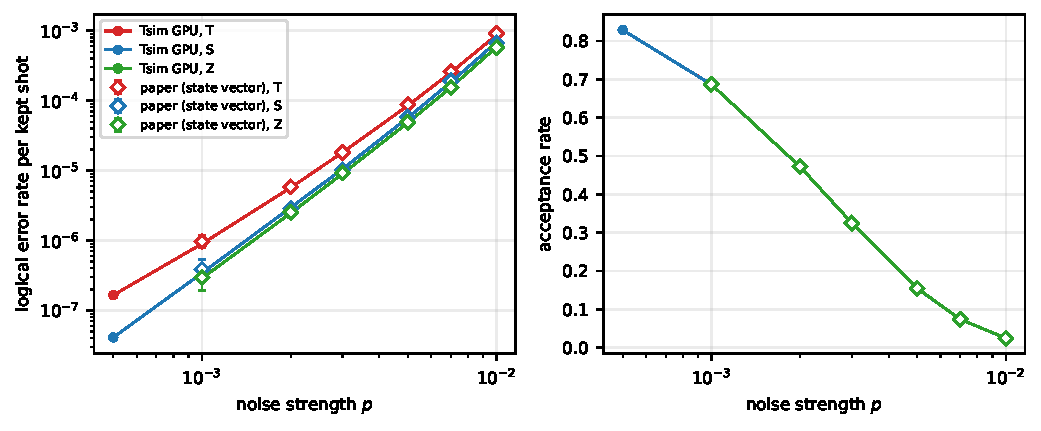
\includegraphics[width=\linewidth]{figures/gidney_cultivation/fig13_t_vs_s.pdf}
\caption*{\textbf{Gidney et al. Fig. 13: cultivating $T$, $S$, $Z$ states ($d=3$, no escape)}\\ \textit{Compute: 1.6 min GPU sampling + 5.3 s compile, 3.1e11 shots, 18 points (NVIDIA GeForce RTX 5090, Tsim a2af975f)}\\ Unitary injection followed by $d=3$ cultivation; every detector postselected; noiseless final logical check (for $T$: $T^{\dagger}$-rotated $Y_L$). Open markers: the paper's state-vector simulation (Zenodo stats.csv). Filled markers: Tsim GPU. $S$ and $Z$ are Clifford proxies of the same circuit.}
\end{figure}

\begin{figure}[h]
\centering
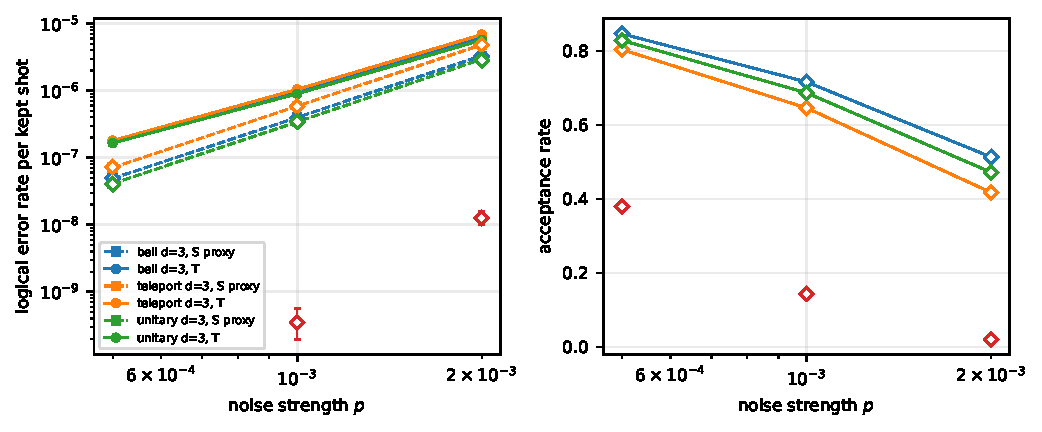
\includegraphics[width=\linewidth]{figures/gidney_cultivation/fig21_inject_only_sampled.pdf}
\caption*{\textbf{Gidney et al. Fig. 21: injection + cultivation, sampled}\\ \textit{Compute: 14.0 min GPU sampling + 6.0 s compile, 2.2e12 shots, 18 points (NVIDIA GeForce RTX 5090, Tsim a2af975f)}\\ Three injection styles with $d=3$ cultivation and unitary injection with $d=5$ cultivation, all detectors postselected. Dashed/squares: the $S$ proxy (the paper's Clifford simulation); solid/circles: real $T$ gates. Open black-edged markers: the paper's Stim data (Zenodo stats.csv, up to $10^{12}$ shots per point). The right panel shows discard rates of the $S$ proxy.}
\end{figure}

\begin{table}[h]
\centering\small
\caption*{\textbf{Gidney et al.: $d=5$ injection + cultivation (no escape)}\\ Each cell: logical error rate of kept shots, errors / kept shots, discard rate, and (Tsim) GPU sampling time.\\ \textit{Compute: not yet sampled}}
\resizebox{\linewidth}{!}{\begin{tabular}{l l l l}
\toprule
$p$ & paper ($S$ proxy, Stim) & Tsim GPU, $S$ proxy & Tsim GPU, $T$ \\
\midrule
0.0005 & 0 (0/3.8e11, disc.\ 0.6208) & -- & -- \\
0.001 & 3.47e-10 (50/1.4e11, disc.\ 0.8560) & -- & -- \\
0.002 & 1.26e-08 (263/2.1e10, disc.\ 0.9792) & -- & -- \\
\bottomrule
\end{tabular}
}
\end{table}

\clearpage

\section{Chase, Labib (2026), Clifft: fast exact simulation of near-Clifford quantum circuits}\label{sec:clifft_inject_cultivate}

\noindent\textbf{arXiv:2604.27058} \quad Study module \texttt{repro/studies/clifft\_inject\_cultivate.py}


Clifft's Fig. 6 plots the logical error rate per kept shot of Gidney's unitary-injection cultivation circuits (no escape) with real $T$ gates and with the $S$ proxy, and their ratio; its Table 2 lists the $d=5$ $T$-gate values at three noise strengths (stratified importance sampling, $9.6\times10^{10}$ shots, 12 machine-hours on a 16-core c6i.8xlarge).

Clifft's circuits are the same as the Gidney study's (the Clifft paper's converter, byte-identical at $p=10^{-3}$), so this study samples nothing itself: it re-plots the Gidney study's unitary-injection points as LER and $T/S$ ratio.

\begin{figure}[h]
\centering
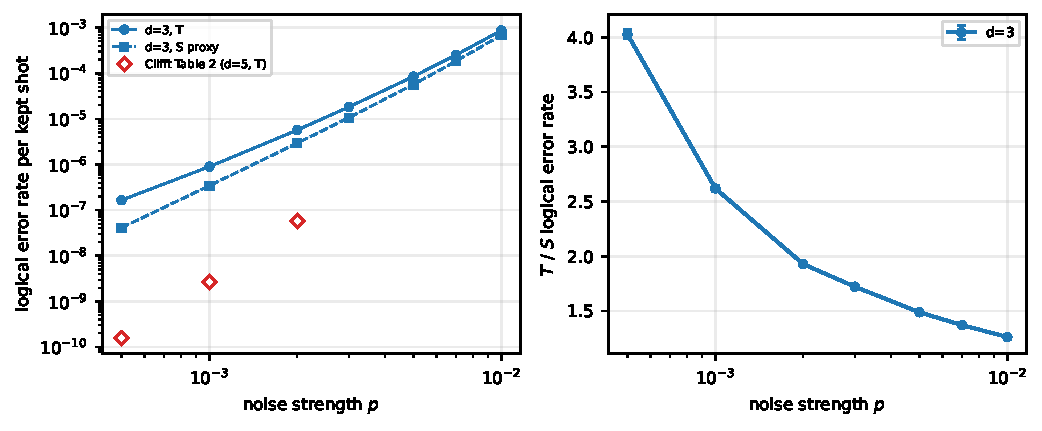
\includegraphics[width=\linewidth]{figures/clifft_inject_cultivate/fig6_t_over_s.pdf}
\caption*{\textbf{Clifft Fig. 6: inject + cultivate, $T$ vs.\ $S$ proxy, and their ratio}\\ \textit{Compute: (Gidney study points): 5.6 min GPU sampling + 4.0 s compile, 9e11 shots, 14 points (NVIDIA GeForce RTX 5090, Tsim a2af975f)}\\ Same samples as the Gidney study (unitary injection). Error bars on the ratio are $\pm1\sigma$ (Poisson). Open diamonds: Clifft's Table 2 $d=5$ values (stratified importance sampling).}
\end{figure}

\clearpage
\end{document}
